\section{Results}
Selected preprocessing / serving / mapping approaches
Survey results
The map application

\subsection{Data preprocessing}

\subsection{Application design}

See \ref{tab:map library comparison} for comparison of mapping libraries.


\begin{table}[h]
	\centering
	\begin{tabular}{ L{0.1\textwidth} | L{0.2\textwidth} | L{0.2\textwidth} | L{0.2\textwidth} | L{0.2\textwidth} } 
		\raggedright
		Library
		& Quality of visualisation
		& Rendering performance
		& License
		& Maintainability
		\\ 
		\hline
		Deck.gl
		& Inconsistent rendering of complex shapes, vector tiles supported
		& Accelerated through webgl, best performace of tested libraries
		\\
		\hline
		Leaflet & Correct rendering, Vector tiles possible through plugins & cell6 \\ 
		\hline
		Mapbox & correct drawing of polygons, raster basemaps & cell6 \\ 
		\hline
		Maplibre & correct drawing of polygons, raster basemaps & cell6 \\ 
		\hline
	\end{tabular}
	\caption{Comparison of mapping libararies}
	\label{tab:map library comparison}
\end{table}

% \begin{table}[h]
% 	\centering
% 	\begin{tabularx}{\textwidth} { 
% 		| >{\raggedright\arraybackslash}X 
% 		| >{\raggedright\arraybackslash}X 
% 		| >{\raggedright\arraybackslash}X 
% 		| >{\raggedright\arraybackslash}X 
% 		| >{\raggedright\arraybackslash}X
% 	}
% 	\hline
% 	asdf & sf & item 11 & item 12 & item 13 \\
% 	\hline
% 	item 21  & item 22  & item 23  \\
% 	\hline
% 	\end{tabularx}
% 	\caption{Comparison of mapping libararies}
% 	\label{tab:map library comparison}
% \end{table}

\subsection{Map usage}

See \ref{fig:Questions 1 and 2} for answers to questions 1 \ref{fig:Question 1} and 2 \ref{fig:Question 2}.

\begin{figure}[H]
	\centering
	\begin{subfigure}[b]{0.5\textwidth}
		\centering
		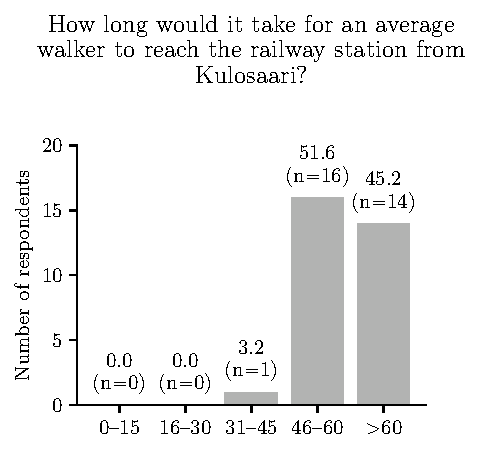
\includegraphics[width=\textwidth]{images/questionnaire/0.pdf}
		\caption{Question 1}
		\label{fig:Question 1}
	\end{subfigure}%
	\hfill
	\begin{subfigure}[b]{0.5\textwidth}
		\centering
		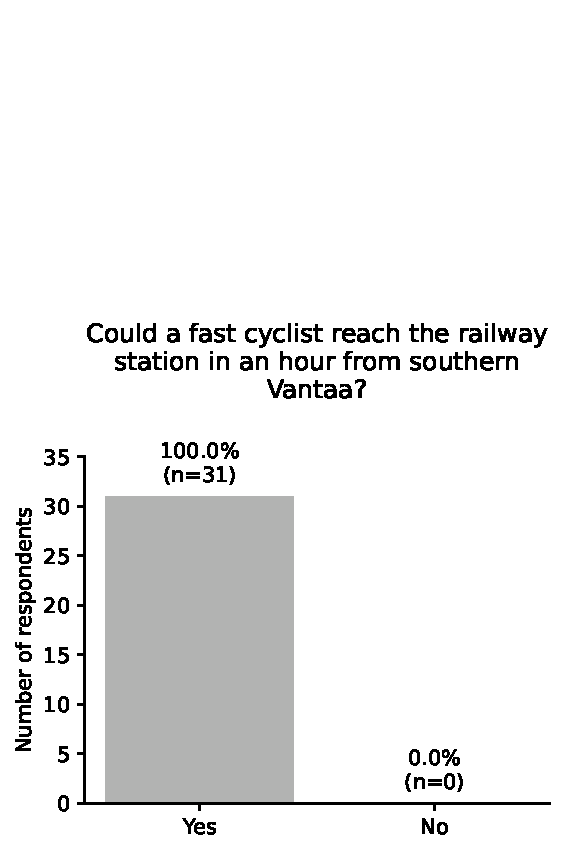
\includegraphics[width=\textwidth]{images/questionnaire/1.pdf}
		\caption{Question 2}
		\label{fig:Question 2}
	\end{subfigure}%
	\caption{Questions 1 and 2}
	\label{fig:Questions 1 and 2}
\end{figure}

\begin{figure}[H]
	\centering
	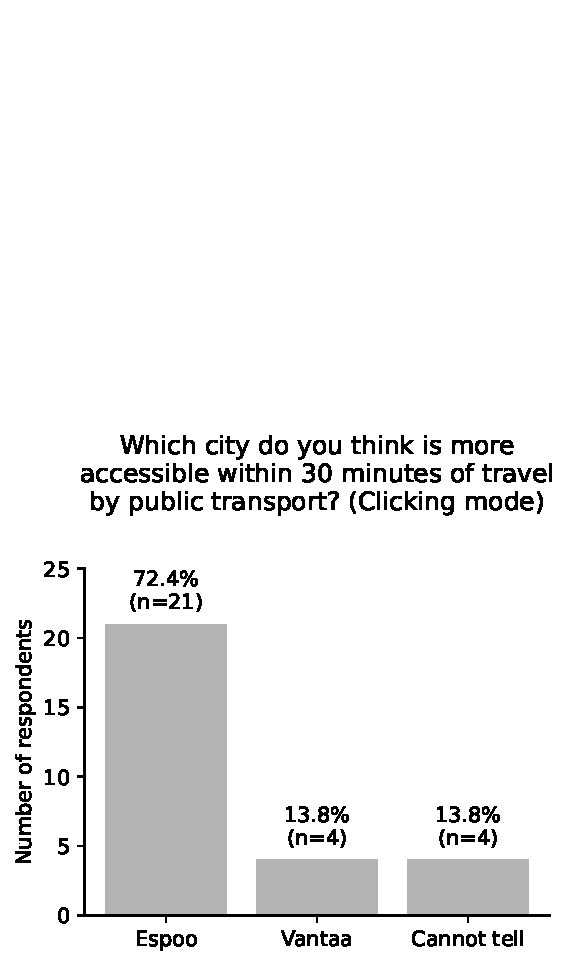
\includegraphics[width=0.5\textwidth]{images/questionnaire/2.pdf}
	\caption{Question 3}
	\label{fig:Question 3}
\end{figure}

\begin{figure}[H]
	\centering
	\begin{subfigure}[b]{0.5\textwidth}
		\centering
		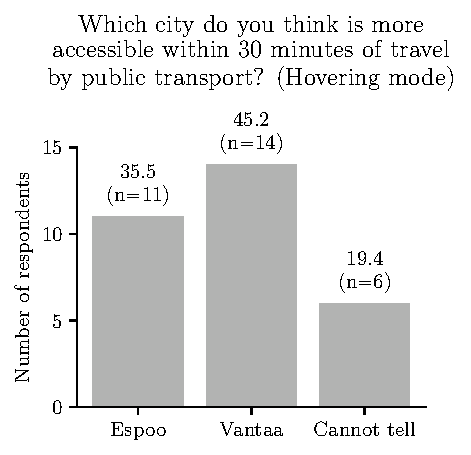
\includegraphics[width=\textwidth]{images/questionnaire/3.pdf}
		\caption{Question 4}
		\label{fig:Question 4}
	\end{subfigure}%
	\hfill
	\begin{subfigure}[b]{0.5\textwidth}
		\centering
		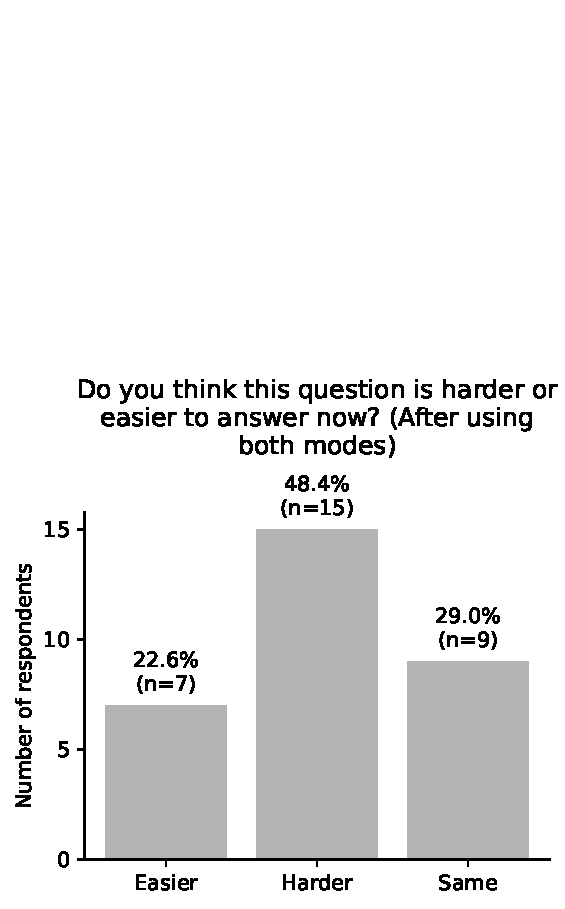
\includegraphics[width=\textwidth]{images/questionnaire/4.pdf}
		\caption{Question 5}
		\label{fig:Question 5}
	\end{subfigure}%
	\caption{Questions 4 and 5}
	\label{fig:Questions 4 and 5}
\end{figure}

% \begin{figure}[H]
% 	\centering
% 	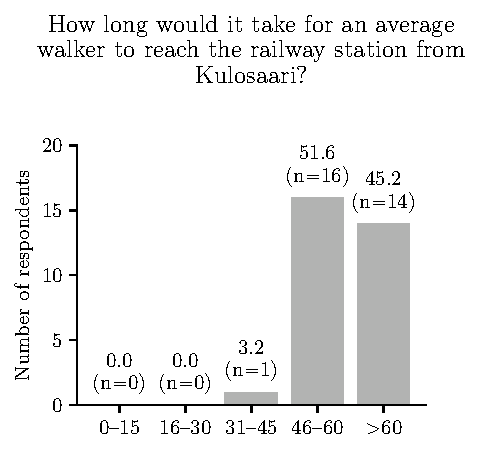
\includegraphics[width=0.75\textwidth]{images/questionnaire/0.pdf}
% 	\caption{Question}
% 	\label{fig:architechture}
% \end{figure}

% \begin{figure}[H]
% 	\centering
% 	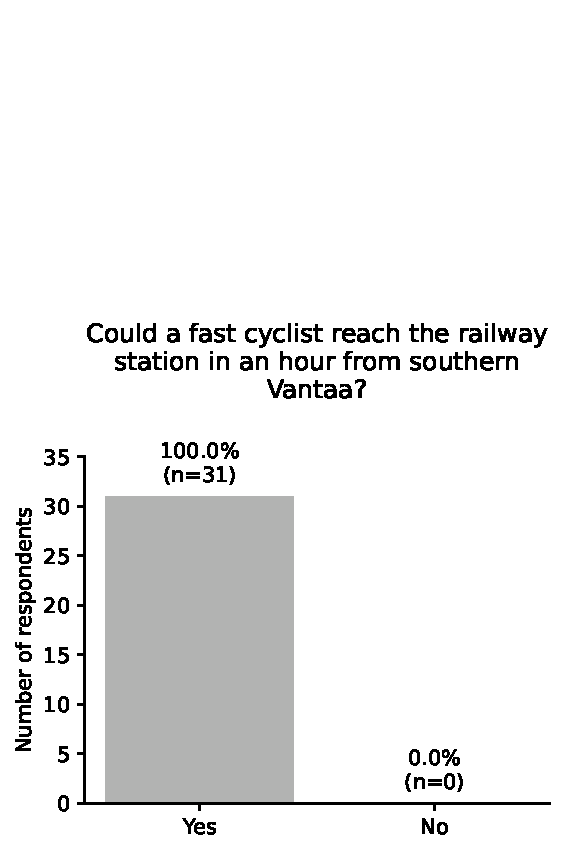
\includegraphics[width=0.75\textwidth]{images/questionnaire/1.pdf}
% 	\caption{Question}
% 	\label{fig:architechture}
% \end{figure}

% \begin{figure}[H]
% 	\centering
% 	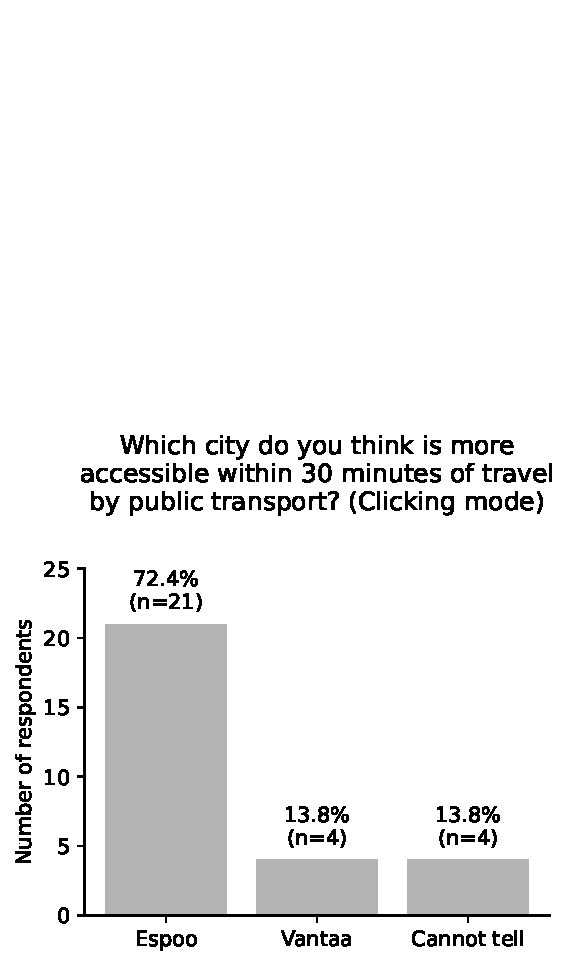
\includegraphics[width=0.75\textwidth]{images/questionnaire/2.pdf}
% 	\caption{Question}
% 	\label{fig:architechture}
% \end{figure}

% \begin{figure}[H]
% 	\centering
% 	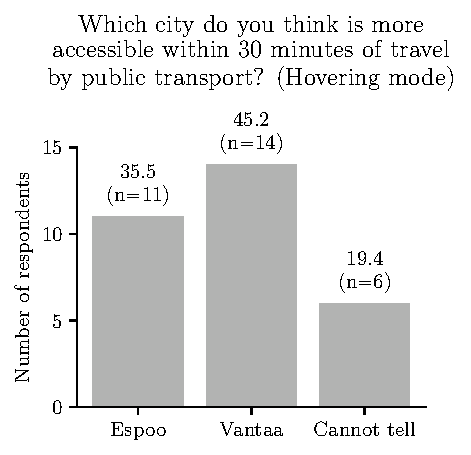
\includegraphics[width=0.75\textwidth]{images/questionnaire/3.pdf}
% 	\caption{Question}
% 	\label{fig:architechture}
% \end{figure}

% \begin{figure}[H]
% 	\centering
% 	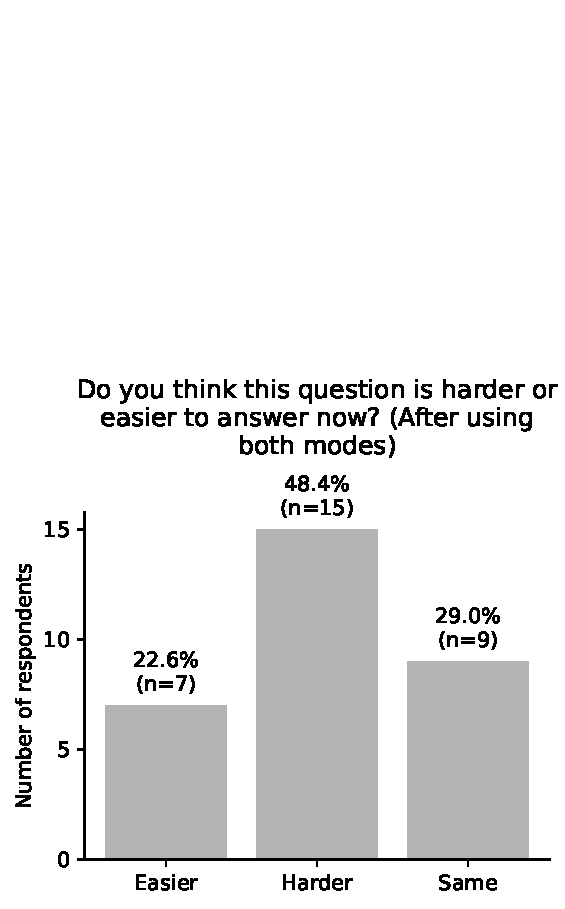
\includegraphics[width=0.75\textwidth]{images/questionnaire/4.pdf}
% 	\caption{Question}
% 	\label{fig:architechture}
% \end{figure}

% \begin{figure}[H]
% 	\centering
% 	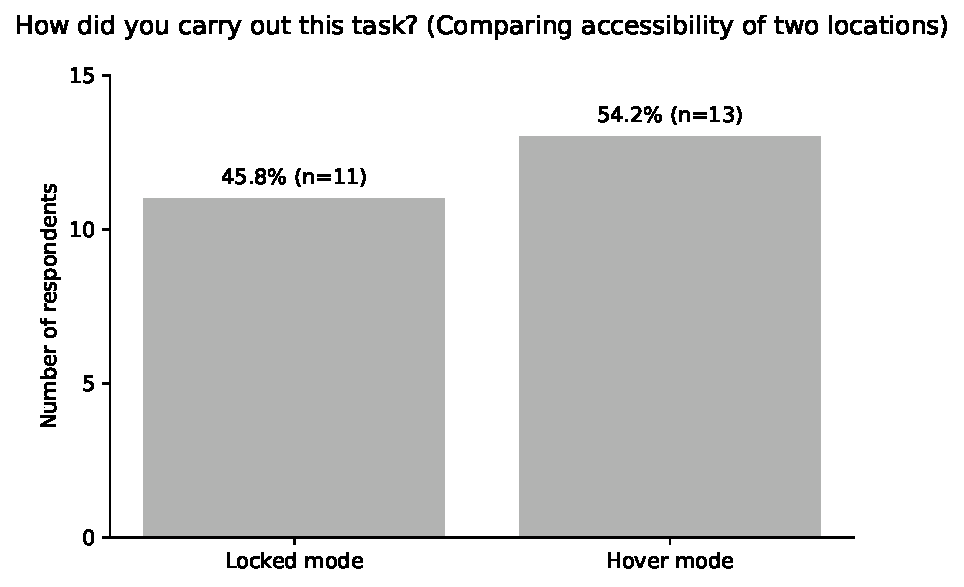
\includegraphics[width=0.75\textwidth]{images/questionnaire/5.pdf}
% 	\caption{Question}
% 	\label{fig:architechture}
% \end{figure}

% \begin{figure}[H]
% 	\centering
% 	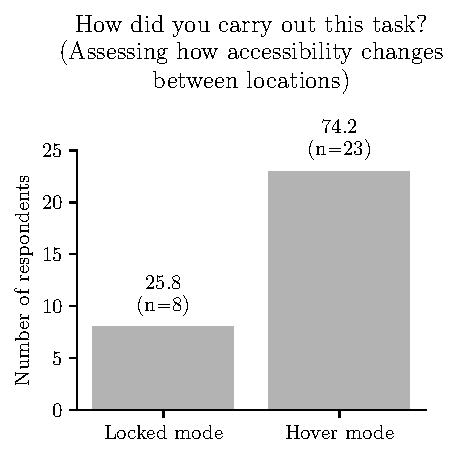
\includegraphics[width=0.75\textwidth]{images/questionnaire/6.pdf}
% 	\caption{Question}
% 	\label{fig:architechture}
% \end{figure}

% \begin{figure}[H]
% 	\centering
% 	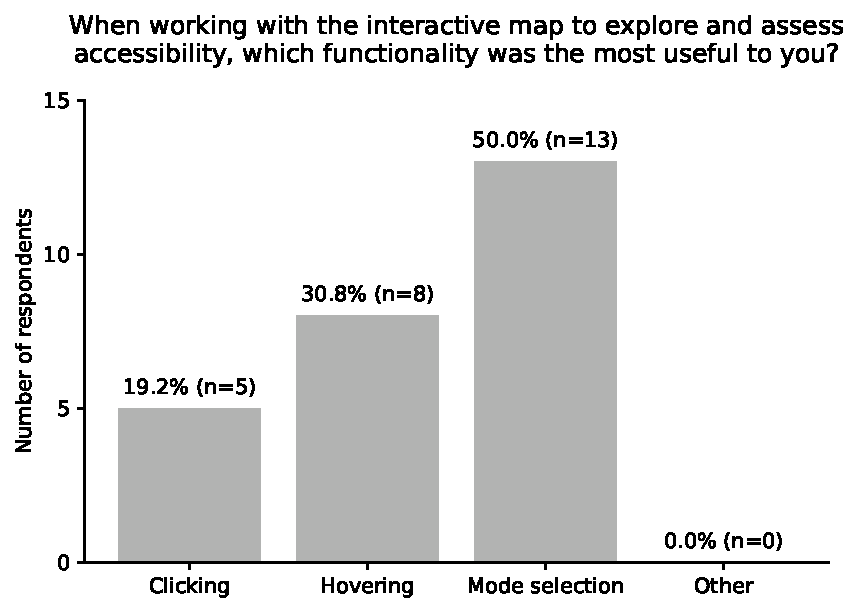
\includegraphics[width=0.75\textwidth]{images/questionnaire/7.pdf}
% 	\caption{Question}
% 	\label{fig:architechture}
% \end{figure}

% \begin{figure}[H]
% 	\centering
% 	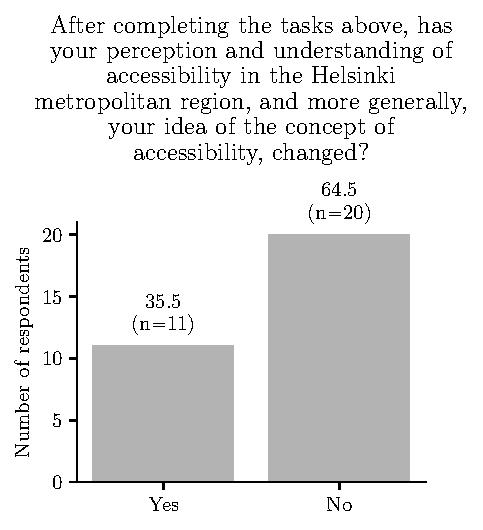
\includegraphics[width=0.75\textwidth]{images/questionnaire/8.pdf}
% 	\caption{Question}
% 	\label{fig:architechture}
% \end{figure}

% \begin{figure}[H]
% 	\centering
% 	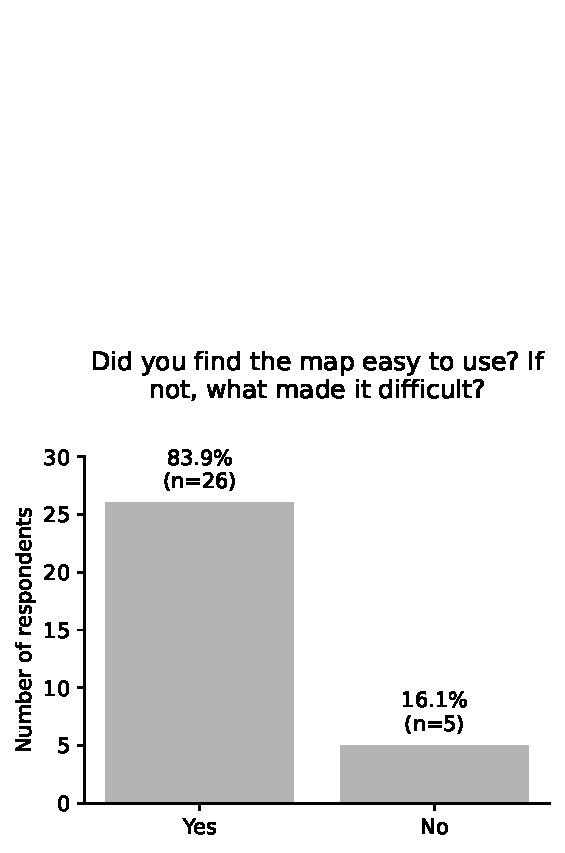
\includegraphics[width=0.75\textwidth]{images/questionnaire/9.pdf}
% 	\caption{Question}
% 	\label{fig:architechture}
% \end{figure}

% \begin{figure}[H]
% 	\centering
% 	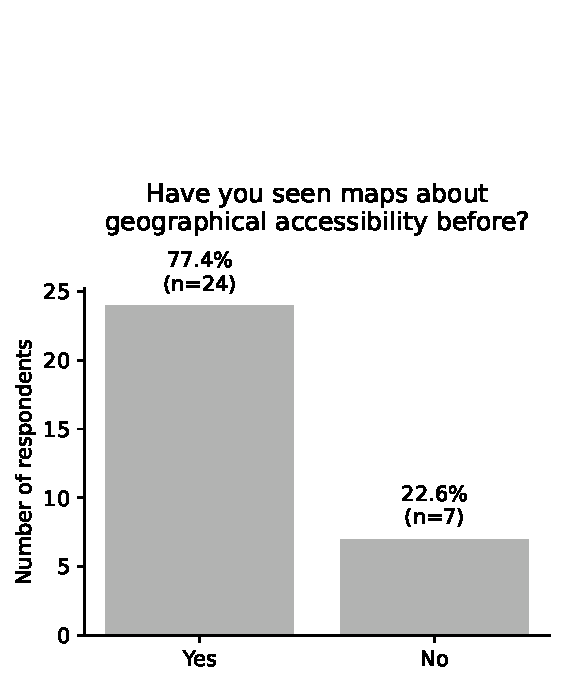
\includegraphics[width=0.75\textwidth]{images/questionnaire/10.pdf}
% 	\caption{Question}
% 	\label{fig:architechture}
% \end{figure}

% \begin{figure}[H]
% 	\centering
% 	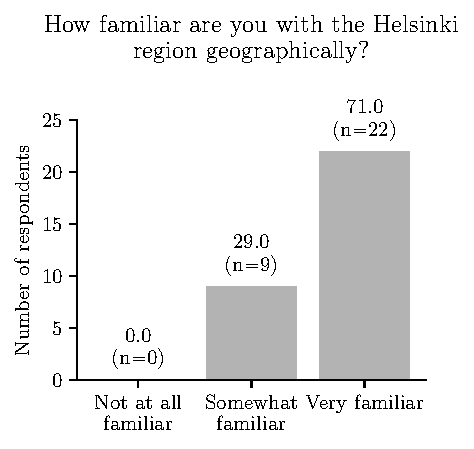
\includegraphics[width=0.75\textwidth]{images/questionnaire/11.pdf}
% 	\caption{Question}
% 	\label{fig:architechture}
% \end{figure}

% \begin{figure}[H]
% 	\centering
% 	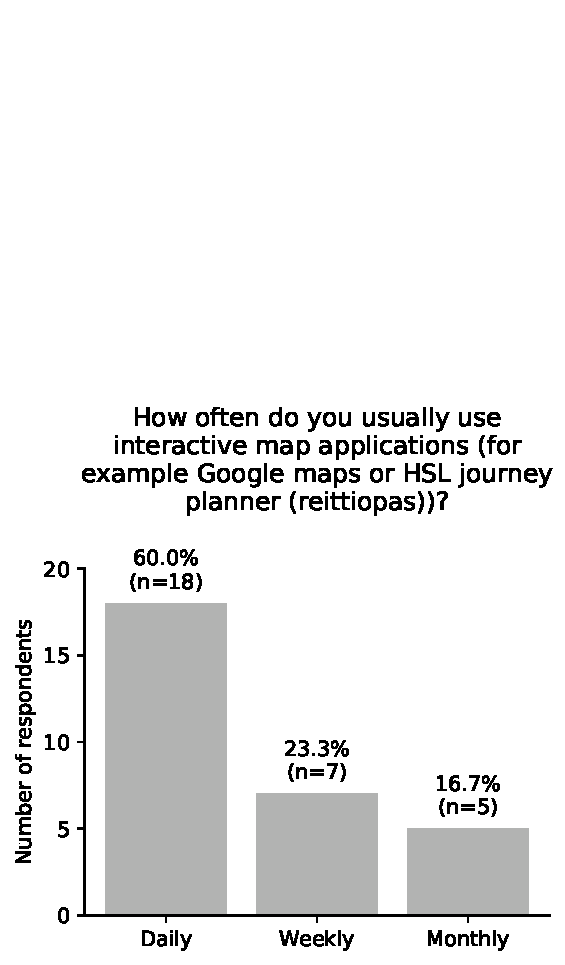
\includegraphics[width=0.75\textwidth]{images/questionnaire/12.pdf}
% 	\caption{Question}
% 	\label{fig:architechture}
% \end{figure}

% \begin{figure}[H]
% 	\centering
% 	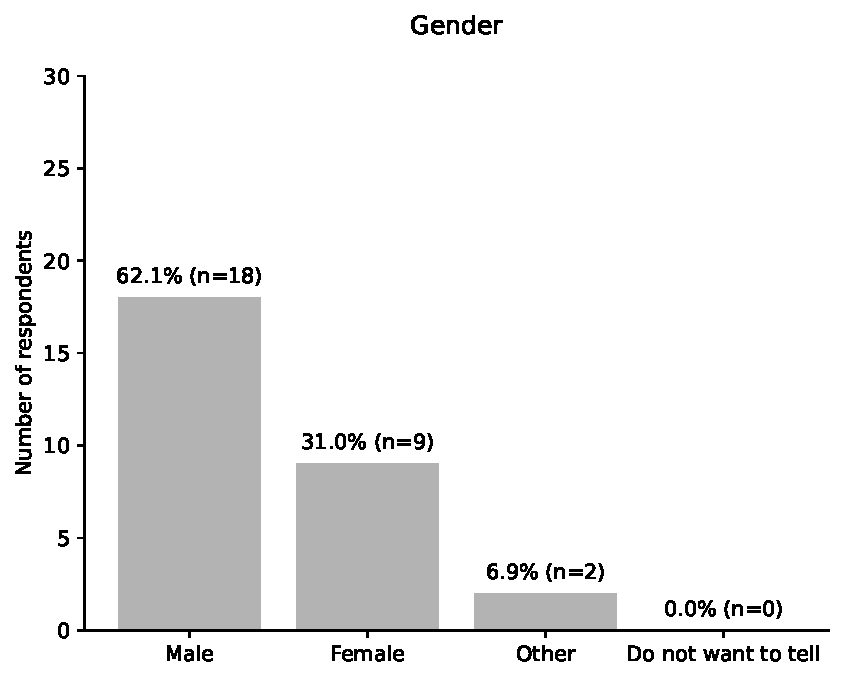
\includegraphics[width=0.75\textwidth]{images/questionnaire/13.pdf}
% 	\caption{Question}
% 	\label{fig:architechture}
% \end{figure}

% \begin{figure}[H]
% 	\centering
% 	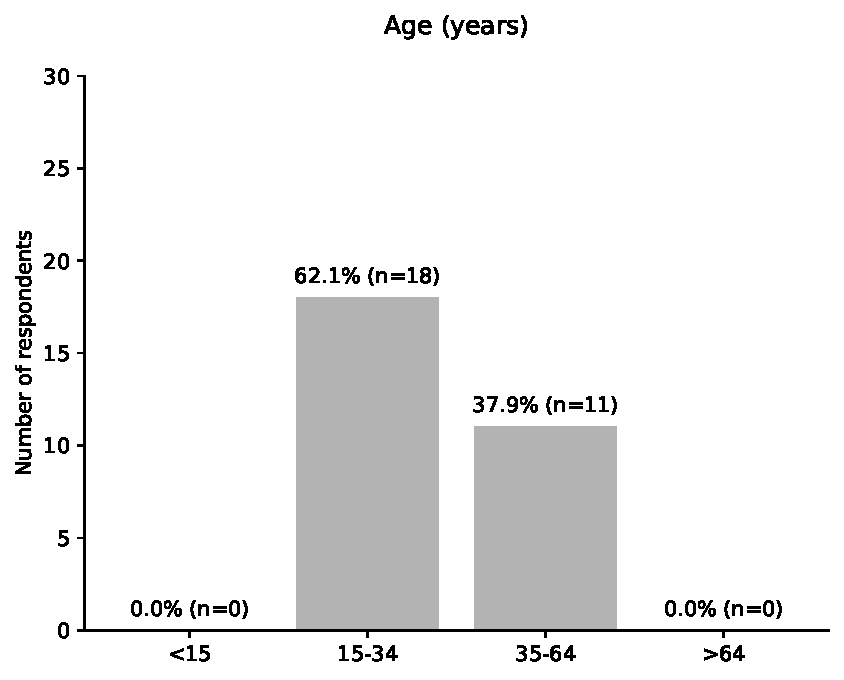
\includegraphics[width=0.75\textwidth]{images/questionnaire/14.pdf}
% 	\caption{Question}
% 	\label{fig:architechture}
% \end{figure}
